

\labday{Wednesday, 02 March 2016}

\experiment{CMOS Array}

\subexperiment{Introduction}
\todo{tbd}

%%%%%%%%%%%%%%%%%%%%%%%%%%%%%%%%%%%%%%%%%%%%%%%%%%%%%%%
\experiment{Experiment Setup}

\begin{figure}[H]
\begin{center}
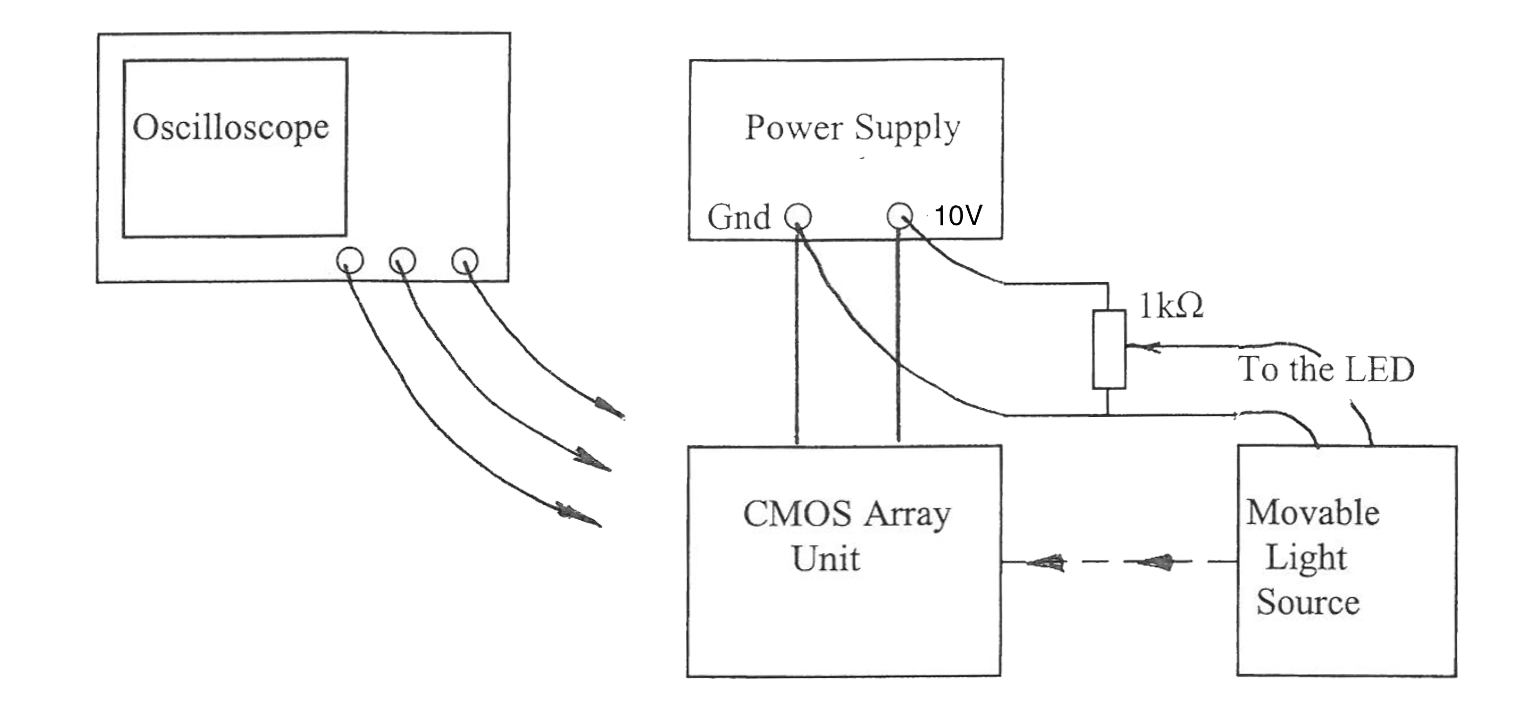
\includegraphics[width=1\linewidth]{LabFour/setup}
\end{center}
\caption{CMOS Array Experiment Setup}
\label{fig:cmossetup}
\end{figure}

\subexperiment{Procedure}

\begin{enumerate}
	\item Arrange and connect up the equipment as shown above.
	\item  Connect the oscilloscope to the CMOS array unit with:
	
			Input 1 to Video Output;

			Input 2 to EOS, End Of Scan;

			Ext. Input to St, Start of Read Out;
			
			Set the time base source to Ext.
	\item On the CMOS array unit set the adjustable controls for the clock frequency, Clk Freq, and the exposure time, Ex Time, to their centre positions and the Gain switch to Low.
	\item With the room darkened and the reading lamp on, switch on the power supply to the LED
and adjust it’s position across the optical bench so that it is in the centre of the bench. Set
up the optical system to focus a small spot on to the centre of the CMOS array. Include an
adjustable iris in the system so that the light level can be altered.

Note, the height of the optical bench may have to be adjusted.
	\item On the oscilloscope set: \\
Time base to 10 msec/division;\\
Input 1 on 1 Volt/division;\\
Input 2 on 5 Volts/division.\\
With the reading lamp on examine the Video output and the EOS displays.
The whole of the array should be seen to be illuminated on the video output display. The
EOS should be at the end of the video read out.
Note, if the room lights are on the illumination level of the array will be so high that the
array stops working.
\end{enumerate}


\subexperiment{Results}

%%%%%%%%%%%%%%%%%%%%%%%%%%%%%%%%%%%%%%%%%%%%%%%%%%%%%%%
\experiment{Clock Frequency}
\subexperiment{Procedure}
\begin{enumerate}
	\item Connect input 2 on the oscilloscope to display the clock, Clk, with the time base at 10 msec.
	\item Alter the clock frequency to see the effect on the video display. Turning the control to the
left reduces the clock frequency and should increase the time for the read out. Increasing
the frequency should reduce the time for the read out.
	\item Reset the clock frequency control to the centre position.

Using the oscilloscope measure the time taken to read out the whole of the array and then
measure the clock frequency by reducing the time base on the oscilloscope until the clock
waveform can be seen. Print out the relationship between the video waveform and the clock
waveform.

Check that the relationship between the clock frequency, the number of pixels and the time
for a complete read out is correct.
	\item On the video trace measure the zero output Voltage level and the peak output voltage level
when the pixels are saturated. The difference is the voltage range from dark to saturated for
the pixels.
\end{enumerate}


\subexperiment{Results}
After connecting the input 2 on the oscilloscope and setting the time base, the clock frequency is set to minimum, see Fig. \ref{fig:clkfreq1}. Altering the clock frequency changes the amount of time needed to read out the CMOS Array, see Fig. \ref{fig:clkfreq2} and Fig. \ref{fig:clkfreq3}.


\begin{figure}[H]
\begin{center}
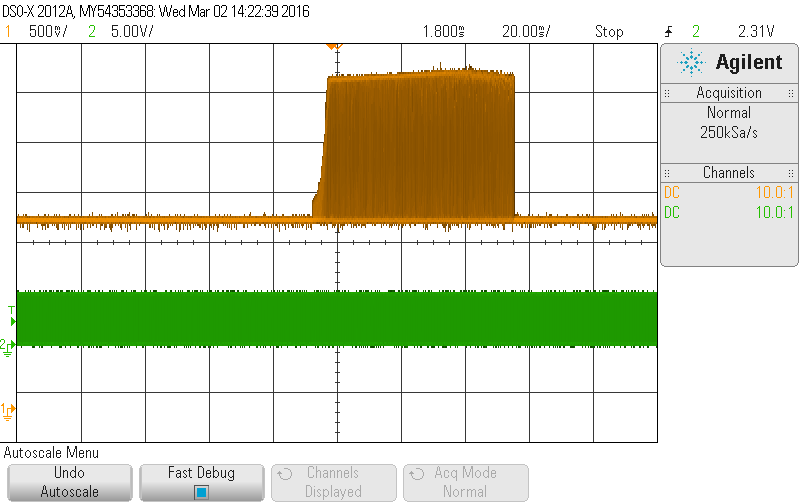
\includegraphics[scale=0.4]{LabFour/scope_53}
\end{center}
\caption{Clock Frequency at minimum}
\label{fig:clkfreq1}
\end{figure}

\begin{figure}[H]
\begin{center}
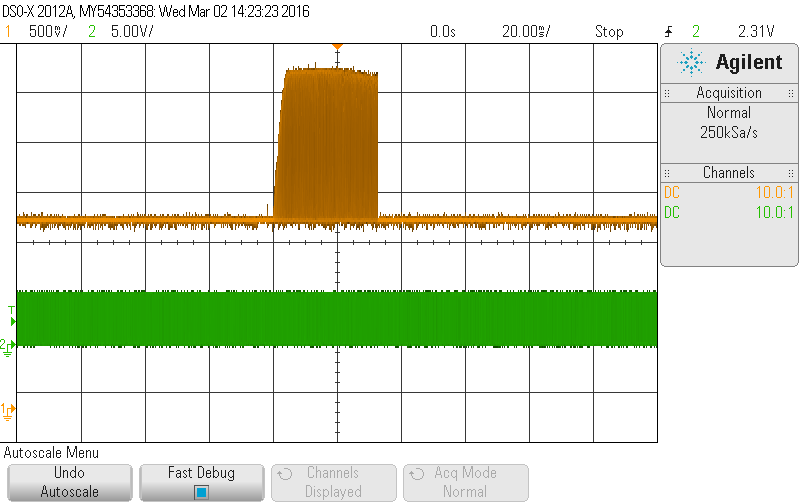
\includegraphics[scale=0.4]{LabFour/scope_54}
\end{center}
\caption{Clock Frequency at centre point}
\label{fig:clkfreq2}
\end{figure}


\begin{figure}[H]
\begin{center}
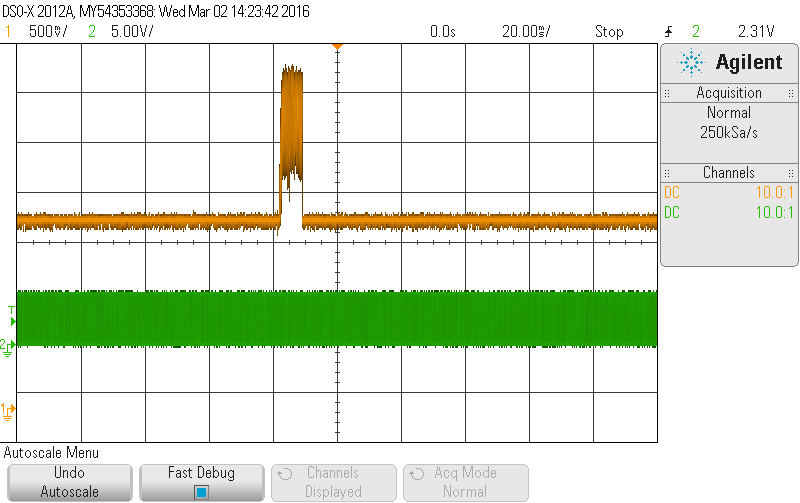
\includegraphics[scale=0.4]{LabFour/scope_55}
\end{center}
\caption{Clock Frequency at maximum}
\label{fig:clkfreq3}
\end{figure}

Now the clock frequency control is again set to the center point and the read-out time of one pixel is measured using the oscilloscope. This results in an read-out time of 39.8 usec for one pixel, see Fig. \ref{fig:clkfreq4} and a read out time of 37.522 msec (\ref{fig:clkfreq5}).


\begin{figure}[H]
\begin{center}
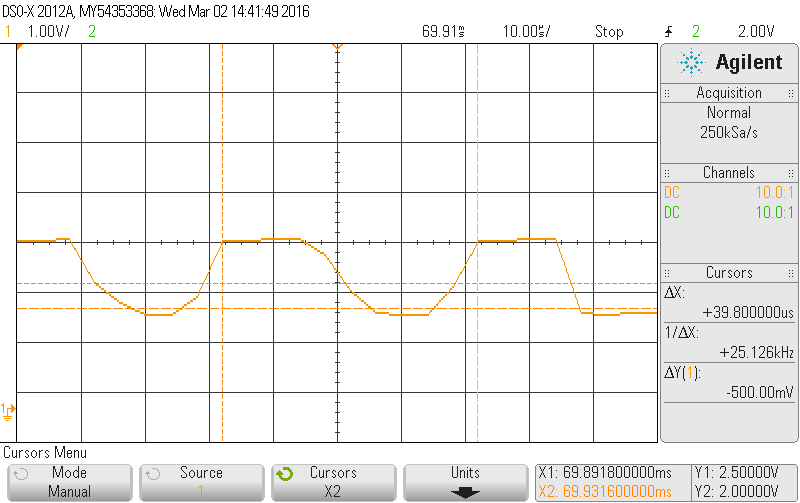
\includegraphics[scale=0.4]{LabFour/scope_61}
\end{center}
\caption{Read Out Time of one pixel, with clock frequency set to centre point}
\label{fig:clkfreq4}
\end{figure}
\begin{figure}[H]
\begin{center}
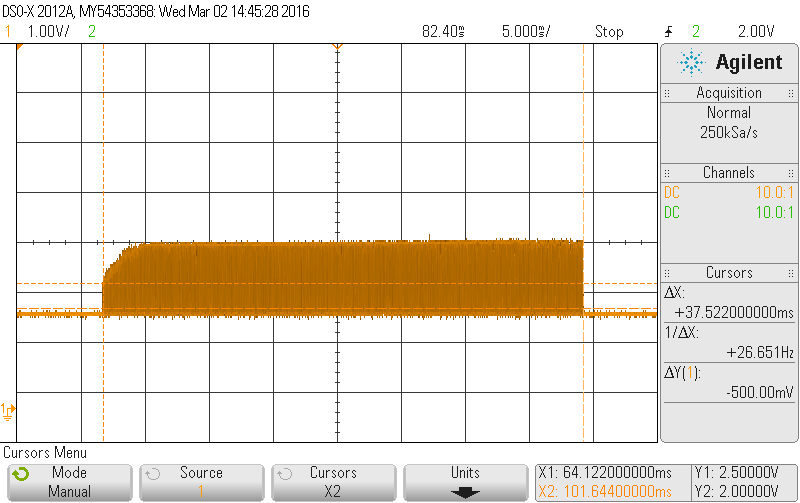
\includegraphics[scale=0.4]{LabFour/scope_62}
\end{center}
\caption{Read Out Time of whole array, with clock frequency set to centre point}
\label{fig:clkfreq5}
\end{figure}

To see the relationship between the clock frequency and the video waveform the time base of the oscilloscope is reduced, as one can see in Fig. \ref{fig:clkfreq6}. The frequency used is 108.695 kHz.

\begin{figure}[H]
\begin{center}
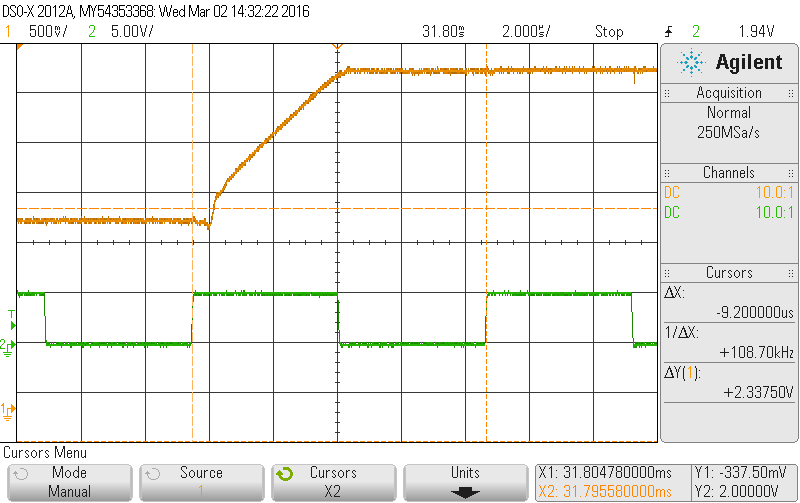
\includegraphics[scale=0.4]{LabFour/scope_59}
\end{center}
\caption{Measuring the clock frequency}
\label{fig:clkfreq6}
\end{figure}

This measurement seems to be correct, but there's a slight deviation from the expected values. According to the data sheet of the CMOS Array the Read-out time for one pixel equals four clock cycles. In our case it results in 4.32 clock cycles for one pixel, which might be the result of a not perfect measurement.\\
Also, the expected read-out time for the whole CMOS Array equals 40.7552 msec (the whole read-out time of the array divided by the read-out time of one pixel), which is slightly more the measured 37.522 msec. This might also be the result of a non-perfect measurement.

Now, the zero output voltage level is measured with saturated pixels (see Fig. \ref{fig:clkfreq7}) and results in 1.8375V.
The voltage range from dark to saturated pixels is 1.53V (see Fig. \ref{fig:clkfreq8}).


\begin{figure}[H]
\begin{center}
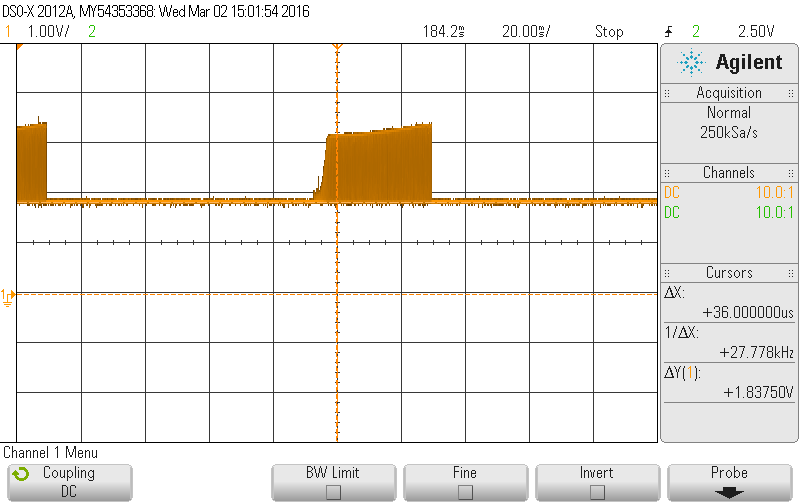
\includegraphics[scale=0.4]{LabFour/scope_63}
\end{center}
\caption{Measuring the Zero Output Voltage Level}
\label{fig:clkfreq7}
\end{figure}

\begin{figure}[H]
\begin{center}
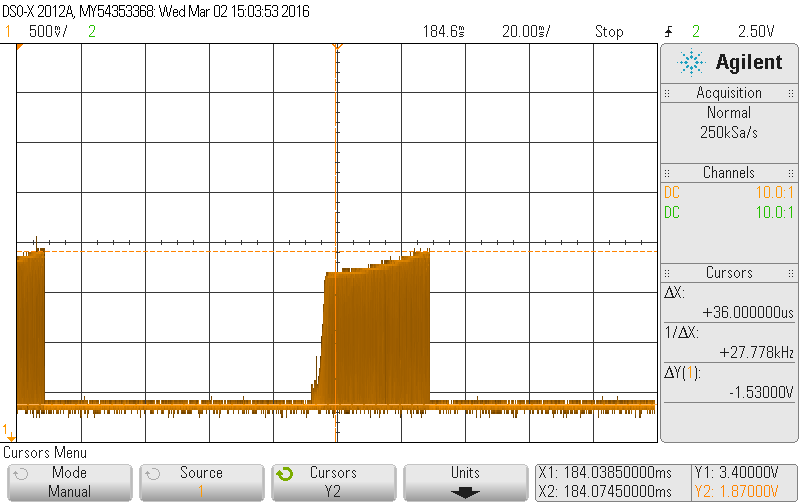
\includegraphics[scale=0.4]{LabFour/scope_64}
\end{center}
\caption{Measuring the Voltage Range from dark to saturated pixels}
\label{fig:clkfreq8}
\end{figure}

%%%%%%%%%%%%%%%%%%%%%%%%%%%%%%%%%%%%%%%%%%%%%%%%%%%%%%%
\experiment{Exposure Time}
\subexperiment{Procedure}

\begin{enumerate}
	\item With the clock and exposure controls at their mid positions set the oscilloscope time base to
50 msec/division. Several read outs from the array should be seen. The exposure time is
the time between the start of successive readouts.

Check that the exposure time is independent of the clock frequency. Reset the clock
frequency to the centre position.

	\item Vary the exposure time control, Ex Time, and view the effect on the oscilloscope screen. In
this system it is possible for the exposure time to be less than the read out time. Reduce the
exposure time until the successive video readouts overlap and note the effect. In a practical
instrument this should not be allowed to happen.

Check that even with low exposure times and low gain too much light stops the CMOS
Array from working.
\end{enumerate}

\subexperiment{Results}
After setting the time base to 50 msec/div we again set all controls to their centre position. Obviously the exposure time is independent from the clock frequency. We verify this by varying the clock frequency and observing the oscilloscope readings.
In Figures \ref{fig:expos1}, \ref{fig:expos2} and \ref{fig:expos3} the effect of varying the exposure time can be seen. 

\begin{figure}[H]
\begin{center}
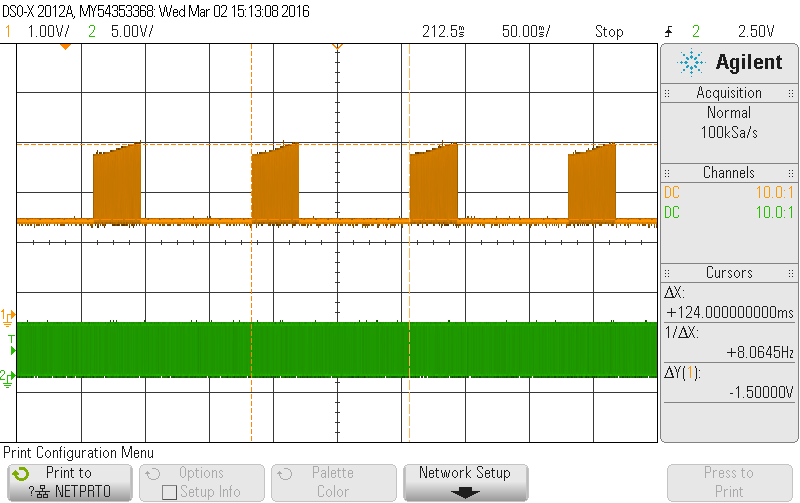
\includegraphics[scale=0.4]{LabFour/scope_65}
\end{center}
\caption{Exposure Time at centre position}
\label{fig:expos1}
\end{figure}

\begin{figure}[H]
\begin{center}
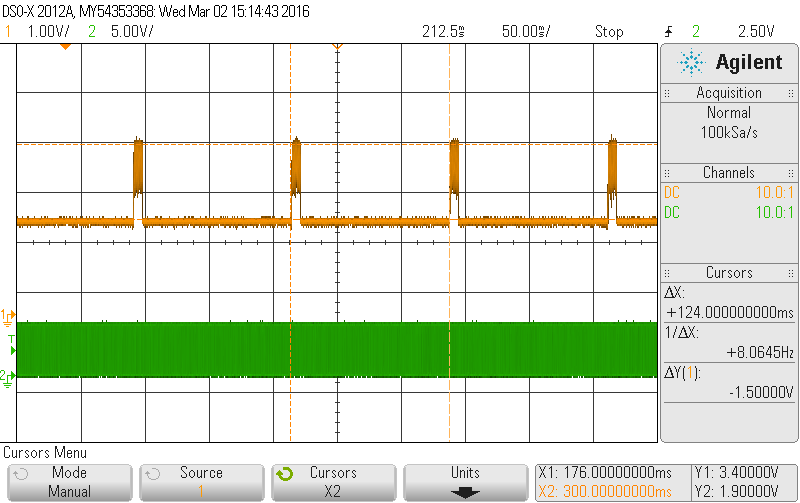
\includegraphics[scale=0.4]{LabFour/scope_67}
\end{center}
\caption{Exposure Time at maximum position}
\label{fig:expos2}
\end{figure}

\begin{figure}[H]
\begin{center}
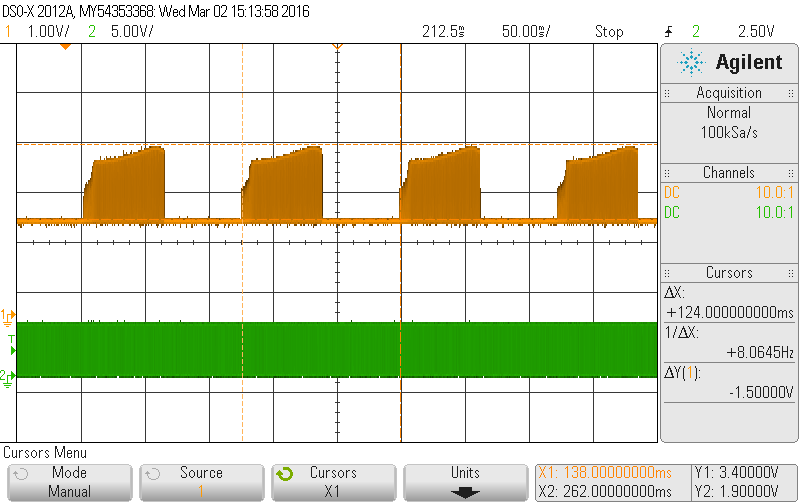
\includegraphics[scale=0.4]{LabFour/scope_66}
\end{center}
\caption{Exposure Time at minimum position}
\label{fig:expos3}
\end{figure}


If the exposure time is reduced too much, successive CMOS Array readings can overlap, as one can see in Fig. \ref{fig:expos4}.
Obviously, this results in a data set that's unusable, since the start and end of each frame is overlapping.
Also, if the CMOS Array is under full illumination while having the exposure and gain set to a low value, the CMOS Array stops working (see Fig. ).

\begin{figure}[H]
\begin{center}
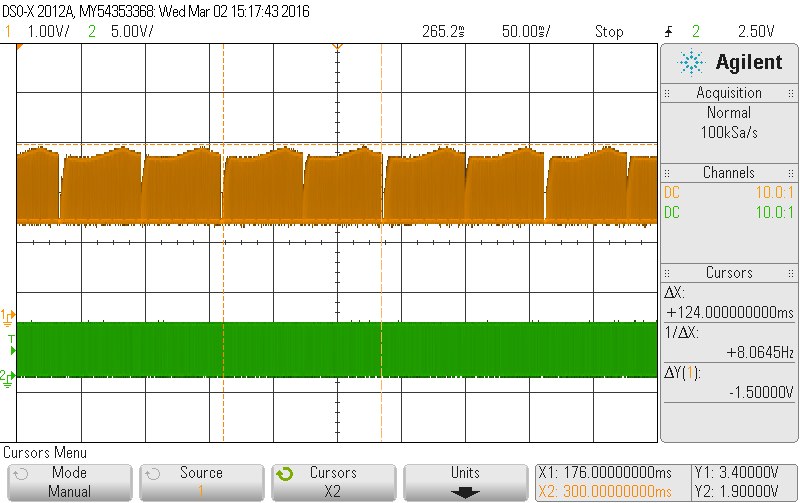
\includegraphics[scale=0.4]{LabFour/scope_68}
\end{center}
\caption{Overlapping Video Readings}
\label{fig:expos4}
\end{figure}

\begin{figure}[H]
\begin{center}
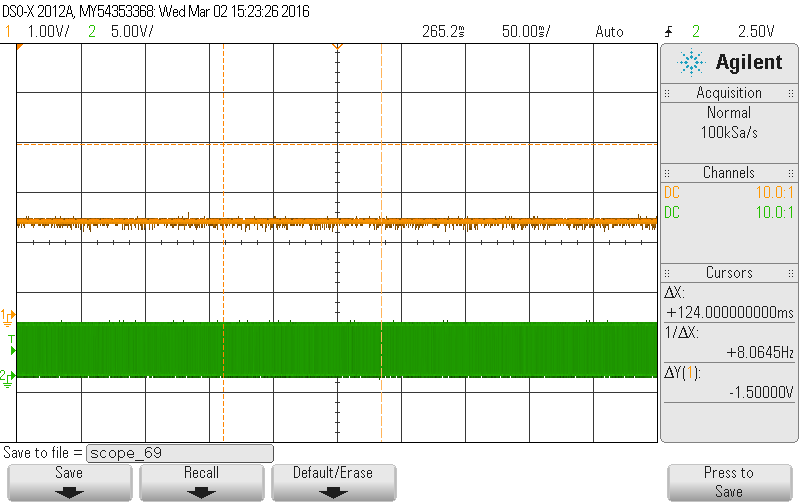
\includegraphics[scale=0.4]{LabFour/scope_69}
\end{center}
\caption{Full Illumination of the CMOS Array while having low gain and low exposure time}
\label{fig:expos5}
\end{figure}

%%%%%%%%%%%%%%%%%%%%%%%%%%%%%%%%%%%%%%%%%%%%%%%%%%%%%%%
\experiment{Spot Illumination}
\subexperiment{Procedure}

\begin{enumerate}
	\item On the array unit set the clock frequency and the exposure time to their centre positions and
the gain to low.

On the oscilloscope:\\
set the time base to 10 msec/division;\\
connect input 2 on the oscilloscope to display EOS..\\
Illuminate the array with a spot at the centre of the array and turn all the lighting in the room
off.
	\item Check, on the oscilloscope, that the illuminated part of the array is near the centre of the
array, if not adjust the position.

Adjust the brightness of the illumination using the iris and the potentiometer until the read
out from the illuminated part of the array can just be seen on the oscilloscope. Switch the
gain to Hi gain and record the change.

Move the display of the illuminated part of the array to the centre of the oscilloscope screen
using the ‘horizontal display’ control.

Expand the display by changing the time base to somewhere between 100usec and 500usec
so that the individual pixel outputs from the charge amplifier can be seen. For one of the
pixels at the centre of the illuminated part of the array measure the magnitude of the output
for both low and high gain. Make sure that the pixel is not being driven into saturation at
high gain. Determine the ratio of high to low gain.

	\item While still examining the individual pixels connect input 2 to the trigger output on the array
unit. Record the relationship between the two traces and comment on why the trigger
output is provided.
\end{enumerate}

\subexperiment{Results}
Again, all controls are set to their centre position, the gain is set to low and the LED is arranged in such a way, that the CMOS Array is illuminated only at its centre.
Figure \ref{fig:spot1} shows the spot illumination at low gain, Fig. \ref{fig:spot2} shows the exact same illumination, but at high gain.



\begin{figure}[H]
\begin{center}
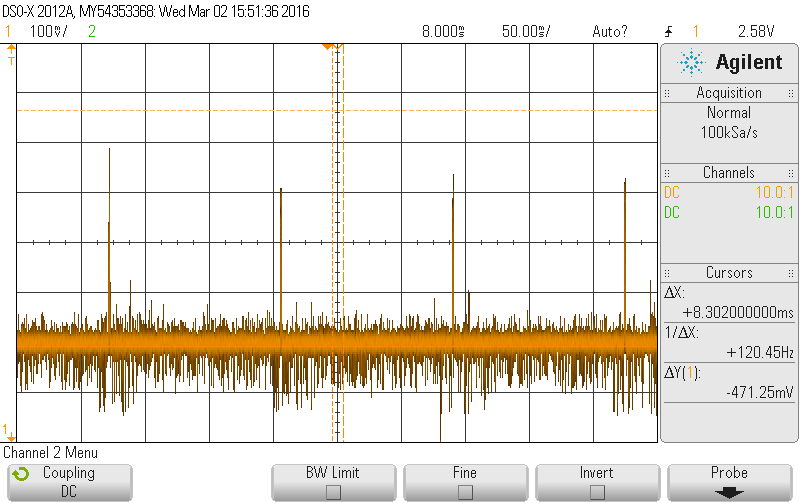
\includegraphics[scale=0.4]{LabFour/scope_79}
\end{center}
\caption{Spot Illuminated CMOS Array at low gain}
\label{fig:spot1}
\end{figure}

\begin{figure}[H]
\begin{center}
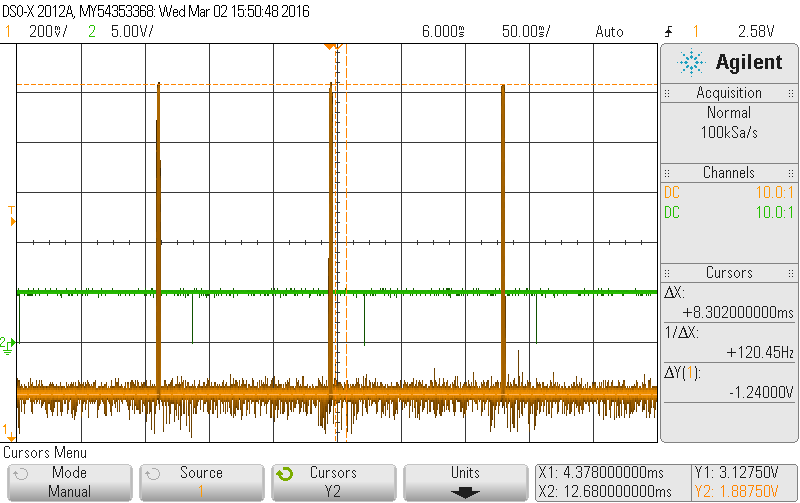
\includegraphics[scale=0.4]{LabFour/scope_78}
\end{center}
\caption{Spot Illuminated CMOS Array at high gain}
\label{fig:spot2}
\end{figure}


In Figure \ref{fig:spot3} and \ref{fig:spot4} the time base was changed to 50 msec/div and 200 msec/div to see the individual pixels.
The magnitude of the output voltage at low gain is 353.75mV and at high gain 1.2275V.


\begin{figure}[H]
\begin{center}
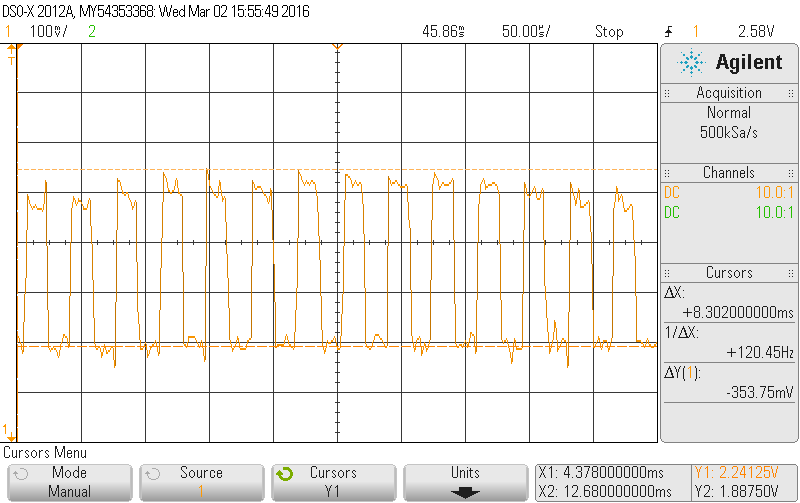
\includegraphics[scale=0.4]{LabFour/scope_81}
\end{center}
\caption{Output voltage magnitude at low gain}
\label{fig:spot3}
\end{figure}

\begin{figure}[H]
\begin{center}
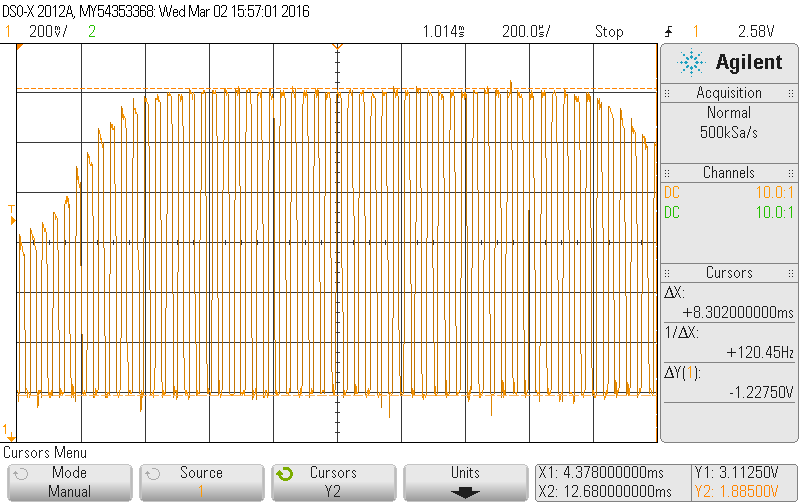
\includegraphics[scale=0.4]{LabFour/scope_82}
\end{center}
\caption{Output voltage magnitude at high gain}
\label{fig:spot4}
\end{figure}
\todo{calculate gain ratio here}



Now the input 2 is connected to the Trigger output at the CMOS Array. The Trigger waveform looks like expected according to the data sheet (see Fig. \ref{fig:spot5}).
\begin{figure}[H]
\begin{center}
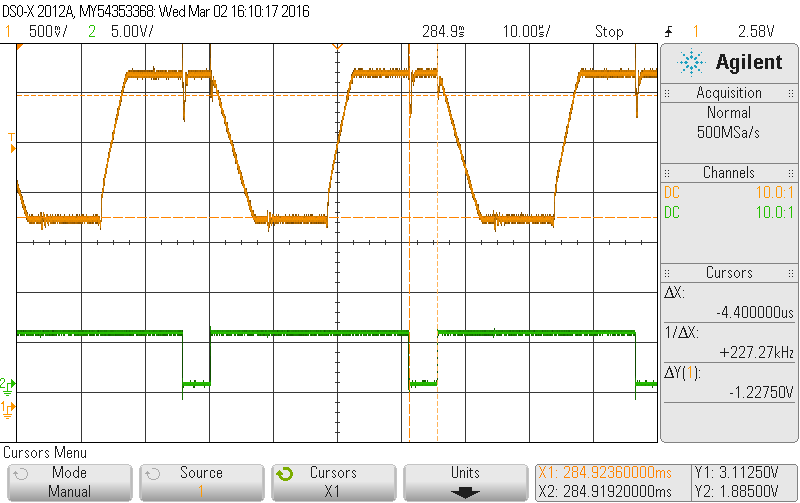
\includegraphics[scale=0.4]{LabFour/scope_87}
\end{center}
\caption{Trigger Output}
\label{fig:spot5}
\end{figure}

The Trigger is used to signal the user or the application, that the CMOS Array reached stable values and is available for readout. 
